\chapter{System Design and Overview}
\paragraph{Overview} % TODO: Review this
 This chapter describes the proposed system from an high level perspective. The purpose of this chapter is in fact to give an overview of how the system modules interact from the point of view of the data flow and use case analysis. Section~\ref{sec:dataflow} describes the system from the perspective of a Data Flow analysis, highlighting the major transformations that produce new levels. Section~\ref{sec:usecases} introduces the main system components from a use case perspective, while section~\ref{sec:modelstructure} focuses on the GAN structure. Details of the chosen architecture are left to Chapter~\ref{sec:networkarch}.


\section{Generative Model Structure}
\label{sec:modelstructure}
\paragraph{Overview} The initial system design was built upon the architecture of Generative Adversarial Networks \cite{gan} from \citeauthor{gan}. Given the problem of generating video-games levels, the need of having a way to control to some extent the  generation process naturally arose. For this reason, we adopted a conditional version \cite{conditionalgan} of the GAN Model, proposed by \citeauthor{conditionalgan}, applied to a more recent \gls{gan} model that is discussed in section \ref{sec:networkarch}.


\begin{figure}[h!]
	\begin{center}
		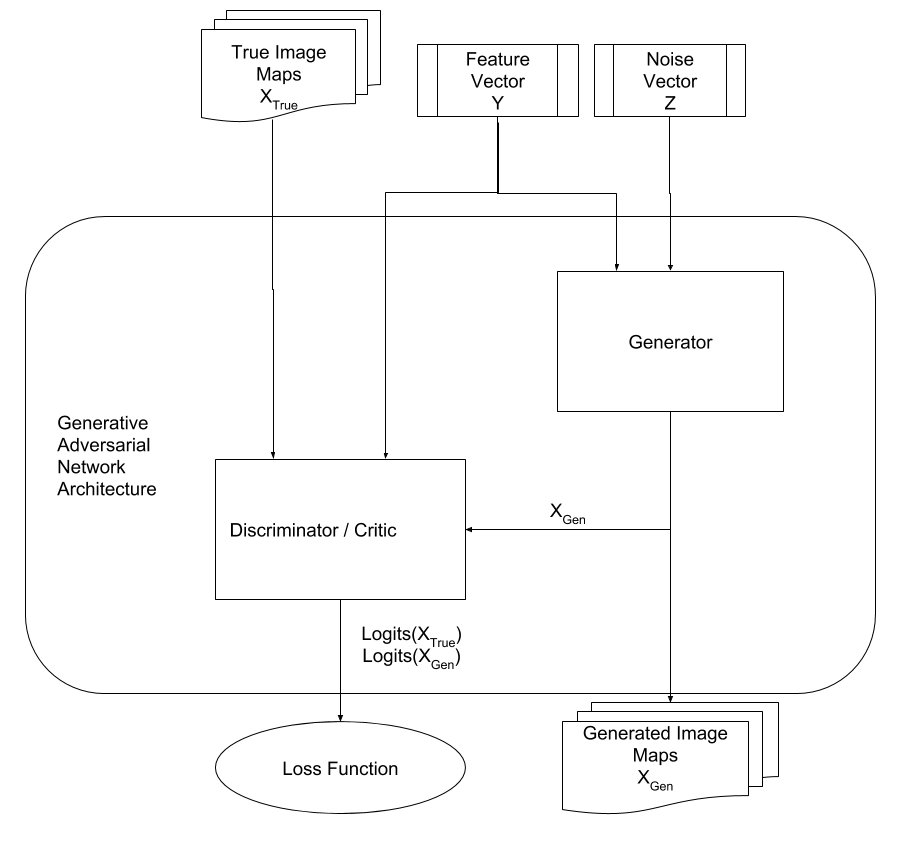
\includegraphics[width=\linewidth]{generative_model_structure}
	\end{center}
	
	\captionsetup{width=\linewidth}
	\caption[System Overview: Generative Model Structure]{ System Overview: Generative Model Structure. A Conditional GAN is composed of a generator model and a discriminative model. The discriminative model takes as input either the Images coming from the dataset or the ones generated by the generative model. Both networks are conditioned by the Y feature vector, while the generator also takes an input a noise vector Z to sample from the data distribution it is approximating. }
	\label{fig:genmodelstructure}
\end{figure}


\paragraph{Conditional GAN Structure} We present in figure \ref{fig:genmodelstructure} the general architecture which defines the inputs and the outputs of the generative model we are using. This structure refers to the Conditional Generative Neural Network we introduced in chapter \ref{sec:introgan}. In particular, figure \ref{fig:genmodelstructure} shows the general working principles of a \gls{gan}: It is composed by two neural networks, namely a Generator and a Discriminator (or Critic, depending on the underlying architecture that is adopted). \\* The input of this subsystem are defined as follows:
\begin{itemize}
	\item $X$: Batch of images having $m$ channels, corresponding to the \glspl{featuremap}.
	\item $Y$: Batch of vectors having one component for each scalar feature considered.
	\item $Z$: Batch of random noise vector, typically sampled from a Uniform or Gaussian distribution.
\end{itemize}

The discriminator network takes as input a vector of images X and a vector of features Y, while the generator network G takes as input a the vector of features Y and a vector of random noise Z, which is used like a "random seed" for generating different samples from the data distribution. We use the subscript "True" or "Gen" to distinguish from the \glspl{featuremap} coming from the input dataset and those that are generated by the generator G.
\\* For what concerns the network outputs, we have that:
\\* $ X_{Gen} = G(Z|Y) $: Samples generated from the generator network
\\* $ Logits(X_{Gen}) = D(X_{Gen}|Y) $: Discriminator output when real samples are in input to the discriminator.
\\* $ Logits(X_{True}) = D(X_{True}|Y) $: Discriminator output with generated samples are provided to the discriminator.
\\* Logits are actually the output of the last layer of the discriminator network before the last \textit{activation function}. A Loss function for either the generator and the discriminator is written upon those values and they are alternatively optimized to train the entire network. All the details are given when we'll describe the chosen GAN Architecture in section \ref{sec:networkarch}.


\section{Use Cases}
\label{sec:usecases}
\paragraph{Overview} This section will describe the main use cases of our system, which are useful for replicating our results. The emphasis is put on how inputs and outputs are used in each case, while the internal structure of the generative model is not represented to simplify the notation. Every figure in this section also describes the function of the dataset metadata introduced in section \ref{sec:metadata_tfrecord} while describing the filtered dataset. In particular the neural network inputs and outputs are limited in a certain range, typically between 0 and 1 or -1 and 1. For this reason, dataset statistics are needed to properly rescale input and output data. Blocks which are written in bold type indicate those inputs and outputs that are of interest for the corresponding use case.

\subsection{Use Case: Model Optimization (Training)}
\label{sec:usecase_train}
\paragraph{} This use case describes the optimization of the model, which is commonly referred as the training phase. This is the phase in which data from the dataset is fed into the model and the loss functions are minimized in order to find the network weights that allow the generation of samples. In the ideal case the generated samples should come from a distribution which is undistinguishable from the true data distribution. In reality, this is limited by both the ability of the discriminator in selecting the features that allow to distinguish true data from artificial one, and the generator ability is misleading the discriminator in its task. Figure\ref{fig:usecase_train} shows that in this use case both the Scalar Features $Y$ and the Feature Maps $Y$ from the dataset are used to train the network. At each epoch the generator network is fed with a random vector $Z$ along with the conditioning vector $Y$. This procedure produces a training loss that is provided to an optimizer that optimizes the network parameters. 

\begin{figure}[h!]
	\begin{center}
		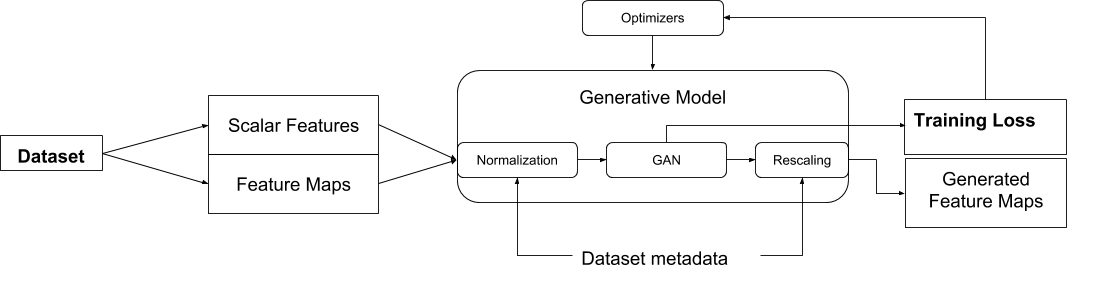
\includegraphics[width=\linewidth]{use_cases_training}
	\end{center}
	
	\captionsetup{width=\linewidth}
	\caption[Use Case: Model Optimization]{Use Case: Model Optimization.}
	\label{fig:usecase_train}
\end{figure}



\subsection{Use Case: Model Validation and Sample Evaluation}
\label{sec:usecase_valid}
\paragraph{} This use case is used to assess the ability of the model to generate new samples on previously unseen feature vectors. This is accomplished by running two different procedures in which only the validation set, composed of samples that are left out from the training phase, is used:
\begin{enumerate}
	\item A \textit{validation loss} is calculated by feeding the discriminator with images $X_{True, Val}$ coming from the validation set and their corresponding feature vector $Y_{Val}$. This approach is often used in standard (non generative) neural networks where it is a good measure of network generalization capabilities. As discussed in section \ref{sec:arch_advantages} in our setting, however, this may not always be a meaningful metric with every proposed underlying architecture. This is usually due to the fact that with many \gls{gan} architectures the loss does not correlate well with the quality sample. %TODO: Citazione necessaria
	\item  A set of \textit{quality metrics} (\ref{sec:evaluation}) are computed directly on the true samples $X_{True, Val}$ and the samples $X_{Gen, Val} = G(Z | Y_{Val}) $ generated by conditioning the network with the same features of $X_{True, Val}$. This is based on the assumption that if the network actually learns a correlation between the $Y$ vector of features and a certain set of features proper to the corresponding $X$ samples, then the true sample and the generated one might show a certain grade of similarity according to the given features. Since this may be a strong assumption, especially in the setting where we are not able to measure what features are actually mapped to each component %TODO: Cita un paper che spiega che è difficile mappare il significato delle features nelle GAN
	 $Y_i$ due to the high dimensionality of the problem, a set of more generic metrics are chosen and presented in section (\ref{sec:evaluation}). Selected metrics should be general enough to express, when averaged on batches of samples, a concept of "sample quality" without directly referring to the features encoded in the $Y$ vector.
\end{enumerate}
 Figure~\ref{fig:usecase_valid} shows how the scalar features from the validation set are used to generate new samples, that are compared to the corresponding true images.

\begin{figure}[h!]
	\begin{center}
		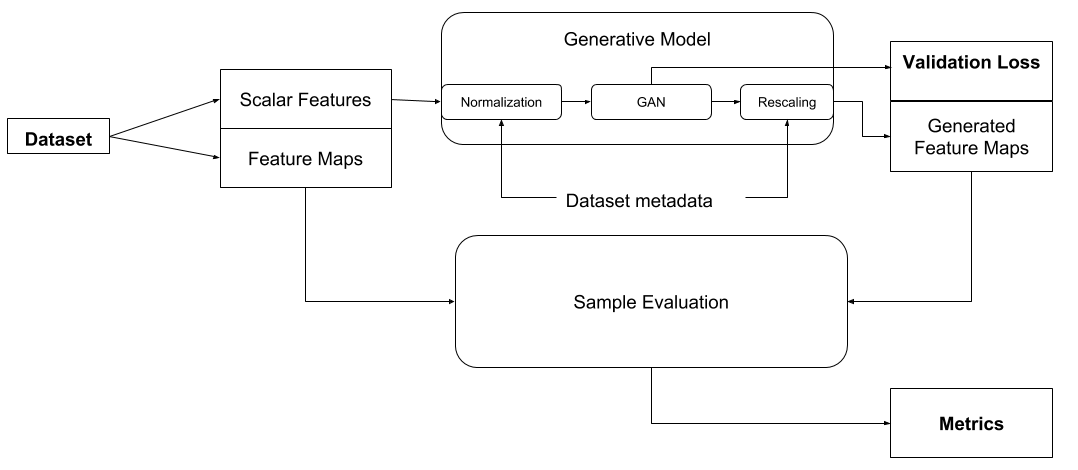
\includegraphics[width=\linewidth]{use_cases_validation}
	\end{center}
	
	\captionsetup{width=\linewidth}
	\caption[Use Case: Validation and Sample Evaluation]{Use Case: Validation and Sample Evaluation.}
	\label{fig:usecase_valid}
\end{figure}

\subsection{Use Case: Sampling or Generation}
\label{sec:usecase_sampling}
\paragraph{} This use case is the one that produces the final output and it is run when a final model is selected. In particular, our system supports several methods for sampling the network in order to generate new levels. \\*
These different sampling methods are motivated in section \ref{sec:sampling}, while in this section we only highlight the differences from an input/output point of view.
The main problem of sampling this network is choosing a feature vector that has enough probability in the distribution 
\begin{itemize}
	%TODO: Go on from here
	\item \textbf{Dataset Sampling}:
	\item \textbf{"Factors" Sampling}:
	\item \textbf{Direct Sampling}:
	\item \textbf{"Content" Sampling}:
	
	
\end{itemize}


\begin{figure}[h!]
	\begin{center}
		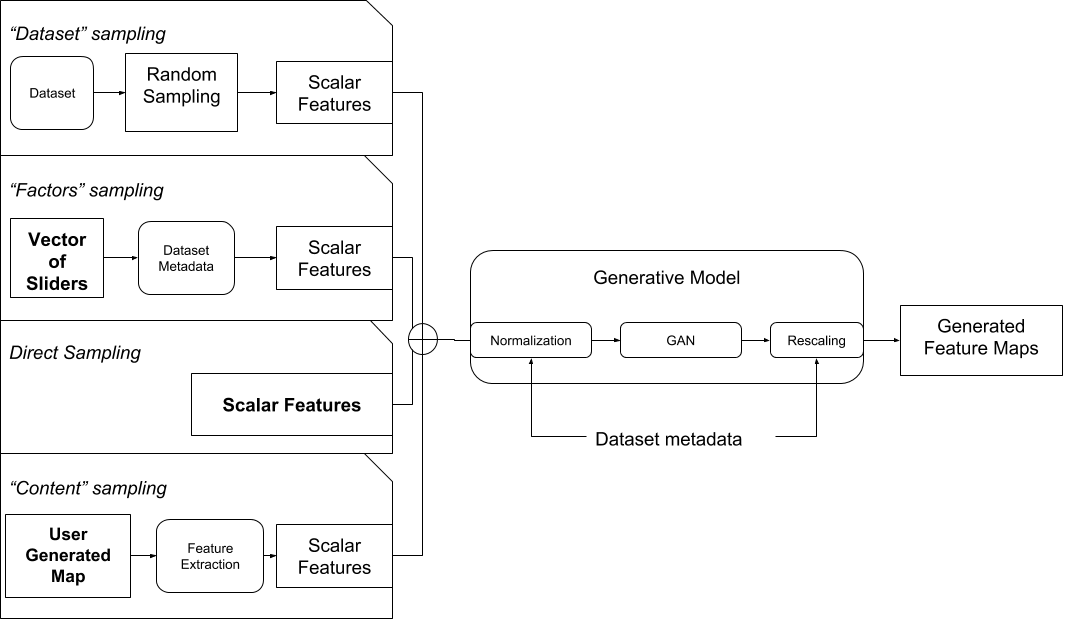
\includegraphics[width=\linewidth]{use_cases_generation}
	\end{center}
	
	\captionsetup{width=\linewidth}
	\caption[Use Case: Sampling or Generation]{Use Case: Sampling or Generation.}
	\label{fig:usecase_sampling}
\end{figure}




\section{Data Flow}
\label{sec:dataflow}
\begin{figure}[h!]
	\begin{center}
		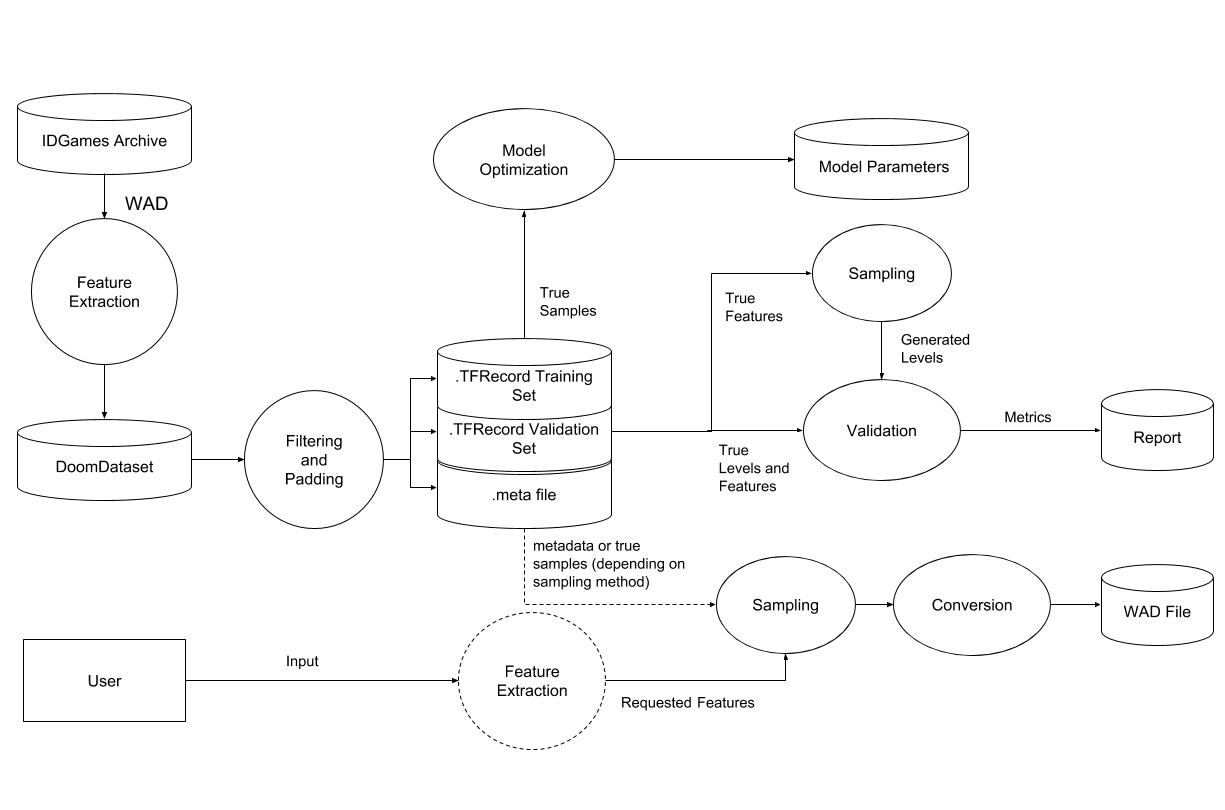
\includegraphics[width=\linewidth]{data_flow_diagram}
	\end{center}
	
	\captionsetup{width=\linewidth}
	\caption[System Overview: Data Flow Diagram]{System Overview: Data Flow Diagram. Disc-shaped blocks represent data archives, circles represent processes and transformations, while the labels on arrows represents intermediate data. Dashed lines represents objects which presence depends on the use case of reference.}
	\label{fig:dataflow}
\end{figure}

\paragraph{Introduction} 
\paragraph{Description} Figure \ref{fig:dataflow} represent the main data transformations for training a new model to produce new DOOM Levels starting from a set of levels collected from the IDGames Archive. Since the scope of this character is to only show a general overview of the system, not every component and transformation is described in detail. The figure is organized as a process developing from left to right. In particular, blocks on the left represent the inputs to the process and blocks on the right boundary are the produced artefacts. \\* 
It is possible to identify three main data paths: The first produces the model parameters and it is identified with the use case "Model Optimization", or "Training" (\ref{sec:usecase_train}), in which the Training Set is used to find a set of network weights that allow to produce new levels. \\* The second one corresponds to the Model Validation and Sample Evaluation use case (\ref{sec:usecase_valid}) in which the model is used to generate new levels using the feature vector taken from the validation set, then the samples from the validation

\section{WAD Editor and Feature Extractor}

\section{Summary}
% We presented a framework for machine learning based level generation that is general enough to be used at least with any generative adversarial network 